\chapter{Untersuchungsmethode}\label{methode}

Wie in den vorhergehenden theoretischen Abschnitten der Arbeit dargelegt wurde, ist es das Ziel der vorliegenden Untersuchung, eine systematische Analyse der ahd. Struktur [\object{dër}\,+\,N] nach  kognitiv-linguistischen, funktionalen und formalen Kriterien durchzuführen. Das vorliegende Kapitel legt die Untersuchungsmethode und die Vorgehensweise offen. Nachdem in Abschnitt \ref{sec:ahd} die Sprachstufe Althochdeutsch und Möglichkeiten ihrer korpuslinguistischen Erschließung ausgelotet werden, erfolgt in Abschnitt \ref{sec:textauswahl} ein Überblick über die Texte, die als Basis für die Untersuchung dienen. Gegenstand von Abschnitt \ref{sec:datenaufbereitung} sind die Schritte der Datenaufbereitung, welche eine genaue Beschreibung des Vorgehens bei der Annotation und eine Beschreibung der Annotationsebenen einschließen. In Abschnitt \ref{sec:analysemethoden} wird das Zusammenspiel von qualitativen und quantitativen Analysemethoden diskutiert sowie der Umgang mit Differenzbelegen erläutert. Das Kapitel schließt mit einer zusammenfassenden Übersicht. 

\section{Das Althochdeutsche und seine korpuslinguistische Erschließung}\label{sec:ahd}

Aus der althochdeutschen Sprachperiode (750--1050) liegen uns nur relativ wenige, zufällig überlieferte und teilweise fragmentarische Textdenkmäler vor \parencite[zur Überlieferungsproblematik s. ausführlich][49--105]{Sonderegger2003}.\footnote{Fleischer bemerkt über die ahd. Quellenlage: \blockcquote[27]{Fleischer2006}{In rein quantitativer Hinsicht ist die Überlieferung des Althochdeutschen innerhalb der altgermanischen Sprachen weder besonders groß (beispielsweise im Vergleich zum Altnordischen oder Altenglischen) noch besonders  klein (beispielsweise im Vergleich mit dem Altniederdeutschen}. Gemessen an heutigen Maßstäben ist die Überlieferungsgröße mit weit unter einer Million Textwörter (s. Abschnitt \ref{sec:ddd}) natürlich als klein einzustufen -- zum Vergleich: das Deutsche Referenzkorpus (DeReKo) beläuft sich auf knapp 47 Milliarden Textwörter (Stand 18.01.2020), s. \url{http://www1.ids-mannheim.de/kl/projekte/korpora.html}.} Man muss sich bei der Arbeit mit althochdeutschem Sprachmaterial daher immer bewusst sein, dass  nur ein sehr kleiner Ausschnitt der damaligen Sprachwirklichkeit abgebildet wird, der darüber hinaus mindestens durch regionale und textsortenspezifische Eigenheiten verzerrt ist  \parencite[27--31]{Fleischer2006}. Aus diesen Gründen können generelle Aussagen über das Althochdeutsche nur mit Vorbehalt gemacht werden. 

Die Fragestellung der vorliegenden Arbeit, ob \object{dër} als Demonstrativ- oder Definitartikel zu klassifizieren ist, setzt eine Analyse des textuellen Kontextes voraus. Zudem wurde in Abschnitt \ref{sec:schema} gezeigt, dass die Entwicklung von \object{dër} auch von systemischen Veränderungen auf Phrasenebene abhängig ist. Ein Korpus des Althochdeutschen, das für solche syntaktischen Fragestellungen angemessen wäre, sollte daher einerseits längere und kohärent zusammenhängende Textabschnitte enthalten. Andererseits muss es hinsichtlich der Variablen Zeit, Region und Textsorte ausbalanciert\footnote{Zum Begriff des \object{balanced corpus}, vgl. \cite[6]{Atkins1992}.} sein, da diese die Ausprägung syntaktischer Strukturen beeinflussen \parencite[74]{Fleischer2011}.\footnote{So zeigt beispielsweise \textcite[47]{Eggenberger1961}, wie metrische Zwänge die Setzung von Subjektpronomina im ahd. Otfrid steuern.} Aufgrund der bruchstückhaften Überlieferungssituation ist ein solcher Korpusaufbau allerdings nicht zu bewerkstelligen. So weist bspw. ein nach Ort und Zeit strukturiertes Korpus des 9. Jahrhunderts, wie \textcite{Fleischer2011} demonstrieren, zahlreiche Lücken auf,  s. Tabelle~\ref{tab:9Jh-matrix}. Auch für die vorhergehenden und nachfolgenden Jahrhunderte gibt es nur fragmentarische Überlieferungen.

\begin{table}
\resizebox{\textwidth}{!}{\begin{tabular}{ccccccccc}
\lsptoprule
  & \multicolumn{2}{c}{Ostfränk.} & \multicolumn{2}{c}{Südrheinfr.} & \multicolumn{2}{c}{Aleman.} & \multicolumn{2}{c}{Bair.} \\
  \cmidrule(lr){2-3}\cmidrule(lr){4-5}\cmidrule(lr){6-7}\cmidrule(lr){8-9}
        & Prosa         & Poesie        & Prosa         & Poesie         & Prosa        & Poesie       & Prosa       & Poesie      \\ \midrule
800--850 & T        & \textminus             & \textminus             & \textminus              & \textminus            & \textminus            & MF         & \textminus           \\
850--899 & \textminus             & \textminus             & \textminus             & O         & \textminus            & \textminus            & \textminus           & \textminus           \\ \lspbottomrule
\end{tabular}}
\caption{Strukturiertes Korpus des 9. Jh. \parencite[75]{Fleischer2011} (T = Tatian, O = Otfrid, MF = Monseer Fragmente)\label{tab:9Jh-matrix}}
\end{table}  

Auch wenn die Quellenlage den Aufbau eines balancierten Korpus nicht zulässt, kann man sich die methodischen Errungenschaften der modernen Korpuslinguistik zunutze machen. Dies bedeutet, dass der Analyse eine systematische Auswahl von Belegen zugrunde liegen sollte: Das Ziel historischer Korpusuntersuchungen muss sein, die vorhandenen Quellen nicht bloß -- wie es \textcite[1310]{Wegera2000} ausdrückt -- \hervor{'steinbruchartig' aus[zu]schlachten}, sondern gesamtheitlich zu analysieren.\footnote{\textcite{Wegera2000} bezieht sich hierbei in erster Linie auf mittelhochdeutsche Quellen. Die Aussage lässt sich jedoch ohne Weiteres auf das Althochdeutsche übertragen.} \textcite[382]{Fleischer2015} präzisiert den damit verbundenen methodischen Paradigmenwechsel:
"`An die Stelle mehr oder minder zufällig zusammengestellter Belege tritt die konsequente und exhaustive Auswertung bestimmter Text(ausschnitt)e in Bezug auf die zu untersuchenden Phänomene"'. Eine solche Arbeitsweise wirkt der Versuchung entgegen, theoretische Entwürfe lediglich auf Basis ausgewählter (und damit oft hypothesenkonformer) Einzelbelege zu modellieren. Zudem schützt sie davor, auffälligen -- weil von der modernen Sprache abweichenden -- Strukturen einen Stellenwert im älteren Sprachsystem einzuräumen, der durch die tatsächliche Vorkommenshäufigkeit vielleicht gar nicht gerechtfertigt werden kann \parencite[383]{Fleischer2015}. Darüber hinaus müssen die für die Untersuchung zentralen linguistischen Kategorien operationalisiert werden  \parencite[113--116]{Lemnitzer2015}. Denn, damit die Klassifizierung eines sprachlichen Ausdrucks nicht das Ergebnis der individuellen Interpretation bleibt, ist es wichtig, möglichst objektive Kriterien zu entwickeln und diese, z.B. in Form von Annotationsrichtlinien, offenzulegen. Die Qualität solcher Richtlinien kann u.a. über sog. \herkur{Inter Annotator Agreements} gewährleistet werden.\footnote{Vgl. hierzu für die vorliegende Arbeit Abschnitt \ref{sec:annotationsschritte}.} 

Wie diese methodischen Anforderungen, also a) die exhaustive Auswertung von längeren ausgewählten Texten/Textausschnitten und b) die Operationalisierung der für die Fragestellung relevanten Kategorien, bei der Untersuchung zum Entwicklung des Definitartikels umgesetzt wurden, dokumentieren die nachfolgenden Abschnitte.


\section{Textauswahl}\label{sec:textauswahl}

Für die Untersuchung wurden die fünf längsten Texte aus der ahd. Sprachperiode ausgewählt: Isidor von Sevilla (I), Monseer Matthäus (M), Tatians Evangelienharmonie (T), Otfrids Evangelienbuch (O) und Notkers Boethius (Buch 1,2) (N), s. Tabelle~\ref{tab:ddd-auswahl}. Die Zusammenstellung ähnelt Oubouzars Datengrundlage \parencite[41--42]{Oubouzar1989}, allerdings mit dem Unterschied, dass die Auswahl um das Matthäus Evangelium aus den Monseer Fragmenten erweitert wurde und Tatians sowie Otfrids Evangelienbuch in ihrer Gesamtheit\footnote{Oubouzars Korpus enthält Kapitel 1--75 aus dem Tatian und Kapitel 2 und 3 aus Otfrids Evangelienbuch.} betrachtet werden.  Die Eigenheiten der einzelnen Texte werden in den nachfolgenden Abschnitten (\ref{sec:isidor}--\ref{sec:notker}) vorgestellt.

\begin{table}[p]
\begin{tabular}{llrc}
\lsptoprule
Text                  & Textsorte      & Ahd. Textwörter & Entstehung \\ \midrule
I                      & Prosa (lat.-ahd.)          &   4.980                  & um 790       \\
M         & Prosa (lat.-ahd.)          & 4.604            & um 810              \\
T & Prosa (lat.-ahd.)          & 37.481                  & um 840              \\
O     & Ahd. Versdichtung          & 60.615               & um 870              \\
N   & Prosa (lat.-ahd. Mischtext) &  17.463               & um 1025             \\ \lspbottomrule
\end{tabular}
\caption{Textauswahl für die Untersuchung}
\label{tab:ddd-auswahl}
\end{table}

\begin{figure}[p]
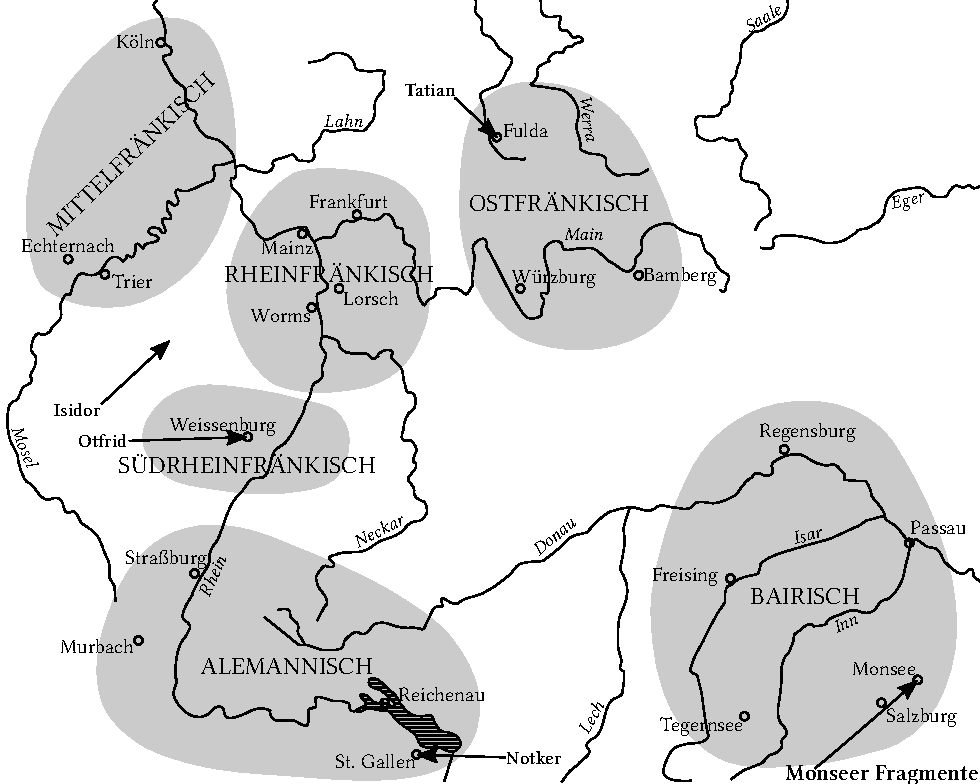
\includegraphics[width=\textwidth]{images/koenig-atlas.pdf}
% %     \begin{tikzpicture}
% %       \node[anchor=south west,inner sep=0] at (0,0) {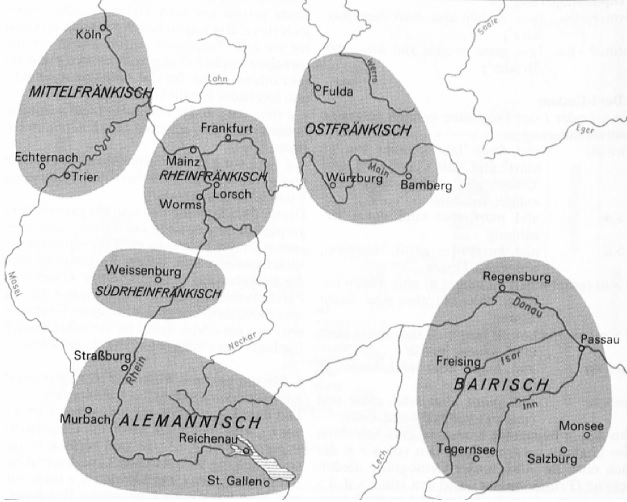
\includegraphics[width=8cm]{images/koenig-atlas.jpg}};
% % 
% %       % \node (T) at (4,5) {\tiny T};
% %       % \node (I) at (1.98,4) {\tiny I};
% %       % \node (O) at (2.4,2.85) {\tiny O};
% %       % \node (N) at (3.18,0.44) {\tiny N};
% %       % \node (M) at (7.45,0.7) {\tiny M};
% % 
% %       \node (T) at (4,5)       {};
% %       \node (I) at (1.98,4)    {};
% %       \node (O) at (2.4,2.85)  {};
% %       \node (N) at (3.18,0.44) {};
% %       \node (M) at (7.6,0.85)  {};
% % 
% %       \node (Ttext) at (3.7,6) {\tiny Tatian};
% %       \node (Itext) at (1,3.5) {\tiny Isidor};
% %       \node (Otext) at (3.3,2.7) {\tiny Otfrid};
% %       \node (Ntext) at (4.35,0.7) {\tiny Notker};
% %       \node (Mtext) at (9,0.5) {\tiny Monseer Fragmente};
% % 
% %       \draw[->] (Ttext) -- (T.center);
% %       \draw[->] (Itext) -- (I.center);
% %       \draw[->] (Otext) -- (O.center);
% %       \draw[->] (Ntext) -- (N.center);
% %       \draw[->] (Mtext) -- (M.center);
% % 
% %     \end{tikzpicture}
\caption {Herkunft der ausgewählten Texte; erweiterte Grafik auf Basis von  \textcite[66]{Konig2015}\label{abb:schreiborte}}
\end{figure}

Das zeitliche Nacheinander der Texte suggeriert ein gewisses Maß an diachroner Kontinuität. Dennoch muss man mit Aussagen über mögliche Entwicklungslinien  vorsichtig sein \parencite[vgl. hierzu auch][158]{Leiss2000}, da die Texte auch eine diatopische Varianz aufweisen, s. Abbildung~\ref{abb:schreiborte}. Insbesondere bei den zeitlich enger beieinander liegenden Texten (Isidor, Monseer Fragmente und bei Tatian) ist daher auch von regional bedingten Einflüssen auszugehen. Der Unterschied von rund 200 Jahren zwischen der Isidorübersetzung und Notkers Boethius ist hingegen groß genug, um diachrone Veränderungen abzubilden.


Doch selbst wenn man die Texte lediglich als isolierte \hervor{Sprachinseln} innerhalb eines spezifischen Zeit-Raum-Koordinatensystems \parencite[157]{Leiss2000} betrachtet, so ist es doch immerhin möglich den jeweiligen Entwicklungsstand eines sprachlichen Ausdrucks (hier: [\object{dër}\,+\,N]) pro Text
zu konstatieren \parencite[vgl. zu diesem Vorgehen auch][29]{Himmelmann1997}. Denn anders als in typologisch-synchronen Untersuchungen, bei denen der zukünftige Entwicklungspfad eines Sprachzeichens nie mit Gewissheit vorhergesagt werden kann, weiß man bei einer historisch-diachronen Untersuchung zumindest, zu welchem  Sprachzeichen sich ein bestimmtes Element entwickelt. Daher sind retrospektiv auch Zwischenstadien in der Entwicklung auszumachen.      


\subsection{Isidor} \label{sec:isidor}

Bei der  ahd. Isidor-Übersetzung (meist verkürzt bezeichnet als \hervor{ahd. Isidor} oder einfach \hervor{Isidor}\footnote{Eine andere Bezeichnung ist \hervor{Pariser Isidor}, gemäß des Aufbewahrungsortes -- die Pariser Nationalbibliothek.}) handelt es sich um eine Übersetzung eines theologischen Traktats des Bischofs Isidor von Sevilla (um 560--636) mit dem Titel \herkur{De fide catholica ex veteri et novo testamento contra Iudaeos}. Sie ist kulturgeschichtlich in die sprachpolitische Missionierungsarbeit Karls des Großen einzuordnen \parencite[vgl.][36--38]{Schlachter2012}. Nach \textcite[VIII][]{Eggers1964} kann das Schriftstück auf Ende des 8. Jahrhunderts datiert werden; die sprachlichen Merkmale deuten auf das Westrheinfränkische hin \parencite{Matzel1970}.\footnote{Für eine intensive philologische Diskussion des ahd. Isidors und der Monseer Fragmente als Teil der sog. Isidor-Gruppe (auch im Vergleich zum ahd. Tatian) sei auf \textcite[17--53]{Schlachter2012} verwiesen.} 

In den insgesamt neun Kapiteln des Isidors steht die lateinische Vorlage dem ahd. Text pa"-ral"-lel innerhalb einer Textseite gegenüber, vgl. Abbildung~\ref{abb:isidor4}.\footnote{Cod. Paris. (Bibl. Nat., Ms. lat.) 2326, p. 2v; 
\url{https://gallica.bnf.fr/ark:/12148/btv1b84260348/f16}; zuletzt aufgerufen am 12.02.2020.} Der Beginn des Traktats ist nur in Bruchstücken als Teil der Monseer Fragmente (s. Abschnitt \ref{sec:monsee}) überliefert; zudem fehlen große Textteile, die vermutlich dem 9. Kapitel folgten \parencite[25]{Schlachter2012}.

\begin{figure}[h]
\begin{center}
  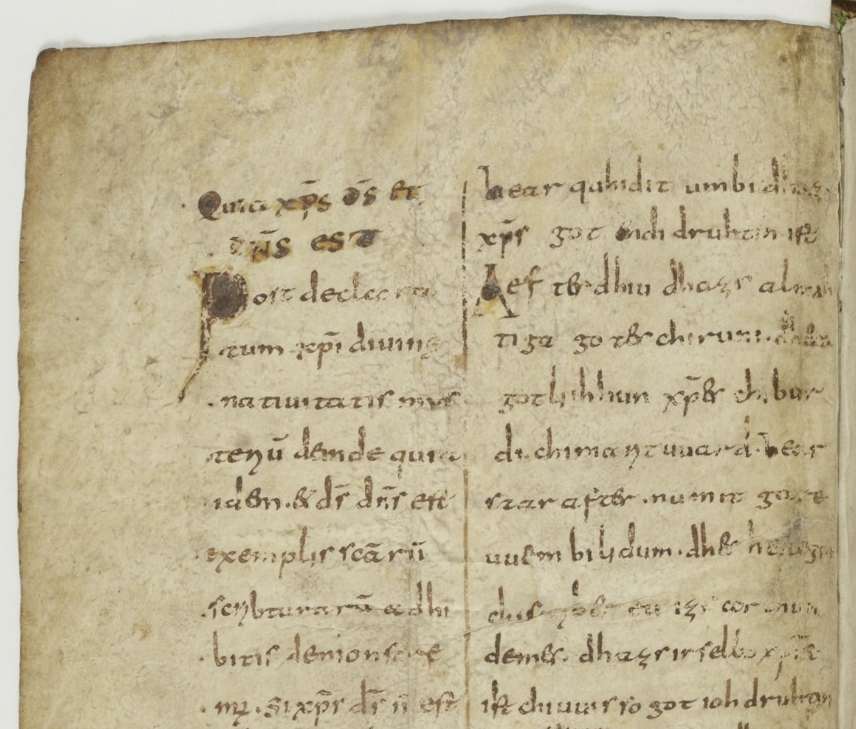
\includegraphics[width=10 cm]{images/isidor-kap-3-ausschnitt.jpg}
  \caption {Der Anfang des 3. Kapitels des ahd. Isidor}
\label{abb:isidor4}
\end{center}
\end{figure} 

%In schwarz-weiß: images/isidor-kap-3-ausschnitt-sw.jpg

Nach \textcite{Matzel1970} wechseln im Schriftstück zwei Übersetzungsstrategien einander ab: Während übersetzte Bibelzitate dem lateinischen Vorbild stark ähneln, werden die auf diesen Zitaten aufbauenden, argumentativen Teile -- zugunsten der \blockcquote[357]{Matzel1970}{theologischen Beweisführung} -- nicht wortwörtlich, sondern meist nur sinngemäß wiedergegeben. Einflüsse der lateinischen Vorlage sind daher vor allem bei den Bibelzitaten zu erwarten \parencites()()[33]{Fleischer2006}[45--46]{Schlachter2012}. Weil der Text sich durch ein stetes Vor- und Zurückverweisen zwischen Bibelstelle und argumentativen Passagen ausweist, ist außerdem damit zu rechnen, dass dem genuinen Demonstrativum \object{dër} als kohärenzstiftendes Mittel eine besondere Rolle zukommt. So zeigt sich bereits in einer Pilotstudie zum 4. Kapitel \parencite[s.][]{Szczepaniak2015}, dass \object{dër} sehr häufig für den anaphorischen Bezug zu abstrakten biblischen Konzepten, etwa \object{drinissa} (\extrans{Dreifaltigkeit}), gebraucht wird. Damit unterscheidet sich Isidor von primär narrativen Textsorten wie den Monseer Fragmenten oder dem größten Teil des ahd. Tatian.   


\subsection{Monseer Matthäus} \label{sec:monsee}

Der Monseer Matthäus ist Teil der Monseer Fragmente. Dabei handelt es sich um eine Sammlung von Einzeltexten, die um 810 im Kloster Mondsee (Nahe Salzburg) ins Bairische übertragen wurden. Überliefert sind Ausschnitte aus den folgenden fünf Texten \parencite{Krotz2003}.


\begin{itemize}
\item Teile von Isidors \herkur{De fide catholica ex veteri et novo testamento contra Iudaeos} 
\item das Matthäus-Evangelium
\item die Predigt \herkur{De vocatione gentium}
\item der Schluss einer unbekannten Predigt
\item die Predigt Nr. 76 des Augustus
\end{itemize}

Den Monseer Fragmenten als Teil der sog. Isidor-Gruppe wird eine hohe Übersetzungsqualität zugeschrieben. Es sind die \blockcquote[129]{Sonderegger2003}{früheste[n] Denkmäler einer selbstständigen althochdeutschen Übersetzungsprosa von erstaunlicher Sprachbeherrschung in der Genauigkeit und Übertragung wie in der eigenen Gestaltung}. 
Leider sind die überlieferten Ausschnitte textlich nicht homogen, was die Vergleichbarkeit untereinander sowie zu anderen Texten einschränkt. Auch in der Überlieferungsqualität sowie der Länge gibt es starke Unterschiede \parencite[s. ausführlich][]{Krotz2002,Krotz2003}. Quantitativ bildet das Matthäus-Evangelium, das mit ca. 120 ahd.-lat. Parallelversen zu knapp zwei Dritteln überliefert ist, das Kernstück der Monseer Fragmente 
\parencites()()[82]{Matzel1970}[26--27]{Schlachter2012}.
Abbildung~\ref{abb:MF-handschrift} zeigt einen Ausschnitt.\footnote{Hannover, Landesbibliothek; \url{https://de.wikipedia.org/wiki/Datei:Mondseer-fragment-3.png}; zuletzt aufgerufen am 12.02.2020.} 

\begin{figure}[h]
\begin{center}
  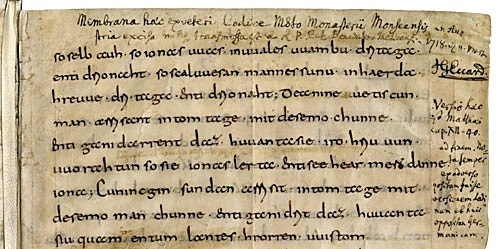
\includegraphics[width=10 cm]{images/MF-handschrift-ausschnitt.jpg}
\caption {Ausschnitt aus dem Monseer Matthäus, Kap. 12}
\label{abb:MF-handschrift}
\end{center}
\end{figure} 

% In schwarz-weiß: images/MF-handschrift-ausschnitt-sw.jpg

% https://de.wikipedia.org/wiki/Datei:Mondseer-fragment-3.png
% laut den Angaben dort gemeinfrei, also einfach verwendbar -- der Link zur
% Quelle funktioniert aber nicht
% -> nach Handschriftencensus gibt es eine Abbildung: Hench, ungezähltes Blatt
% vor Titel [= (b) Bl. 2r]; habe ich aber im verlinkten Faksimile nicht gefunden
%, V.40 bis Kap. 13, V.1. (Hannover, Landesbibl., Ms. I 20b, Bl. 2r)

%alternativ: http://digital.onb.ac.at/RepViewer/viewer.faces?doc=DTL_5736858&order=1&view=SINGLE

Der Matthäus-Text stellt ein interessantes Vergleichsobjekt dar, weil er  einerseits stilistisch mit dem etwas älteren Isidor verwandt ist \parencite{Hench1893,Lippert1974} und andererseits Teile davon auch im jüngeren ahd. Tatian vorkommen. Für die nachfolgende Untersuchung wird daher der Matthäus-Text aus den Monseer Fragmenten als Textgrundlage ausgewählt und in Anlehnung an die Terminologie von \textcite{Lippert1974} als \hervor{Monseer Matthäus} bezeichnet.
  
\subsection{Tatian}\label{sec:tatian}

Auch bei der Evangelienharmonie des Tatian (nachfolgend auch kurz: \hervor{(ahd.) Tatian}) handelt es sich um einen Übersetzungstext. Dem lateinischen Original ist die ahd. Übersetzung nach dem \hervor{Prinzip der korrespondierenden Zeilen} \parencite[43]{Fleischer2011} parallel gegenübergestellt \parencite[vgl. hierzu auch][128]{Masser1997}. Der Text ist vermutlich in der ersten Hälfte des 9. Jhs. entstanden; die Datierungsvorschläge reichen von 830 \parencite[LXX]{Sievers1961} bis 850 \parencite[127]{Sonderegger2003}. Einig ist sich die Forschung, dass die Handschrift aus dem Kloster Fulda stammt und die Sprache als ostfränkisch zu klassifizieren ist. Mehrere Übersetzer waren daran beteiligt \parencite[s.][31]{Masser1994}. In Abbildung~\ref{abb:tatian-hand} ist ein Auszug der ersten Zeilen abgebildet.\footnote{St. Gallen, Stiftsbibliothek, Cod. Sang. 56, p. 262 –
Evangelienharmonie des Tatian; \url{https://www.e-codices.unifr.ch/de/csg/0056/25/0/Sequence-262}; zuletzt aufgerufen am 12.05.2020}

\begin{figure}[h]
\begin{center}
  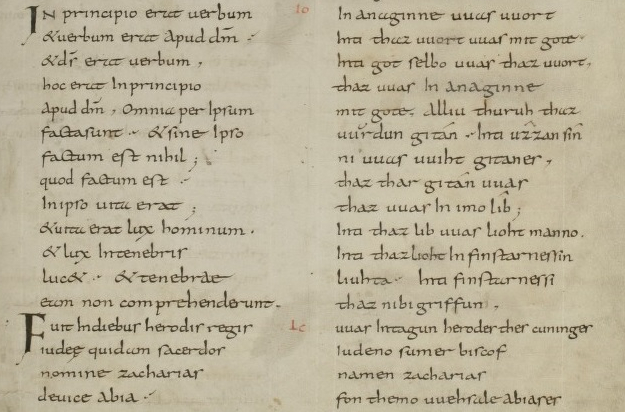
\includegraphics[width=10 cm]{images/tatian-handschrift-ausschnitt.jpg}
\caption {Auszug aus dem Tatian (\extrans{am Anfang war das Wort...})}
\label{abb:tatian-hand}
\end{center}
\end{figure} 

%In schwarz-weiß: images/tatian-handschrift-ausschnitt-sw.jpg

% http://www.e-codices.unifr.ch/de/csg/0056/25/0/Sequence-262
%% Verwendung: http://www.e-codices.unifr.ch/de/about/terms
%% nicht kommerziell mit cc-by; kommerziell bedarf schriftlicher Genehmigung
%% Ort, + Bibliothek, + Signatur, + Seitenzahl (www.e-codices.unifr.ch).
% Beispiel: 
% Engelberg, Stiftsbibliothek, Cod. 14, f. 12r (www.e-codices.unifr.ch).

Im Gegensatz zu dem ahd. Isidor und den Monseer Fragmenten wird der Ta"-ti"-an-Bi"-ling"-ue eine relativ starke Lateinabhängigkeit attestiert \parencites(){Lippert1974}[128]{Sonderegger2003}. Das Paradebeispiel für den lat. Einfluss ist der Umgang mit dem Ablativus absolutus. Die Konstruktion wird im Tatian fast immer in eine parallele Dativform überführt -- eine Strategie, die in den anderen ahd. Schriftstücken kaum zu beobachten ist \parencite[145f]{Lippert1974}. Daher kann man davon ausgehen, dass es sich bei diesem \hervor{absoluten Dativ} um eine nicht genuin ahd. Struktur handelt \parencite[zur vertiefenden Diskussion s.][39--40]{Fleischer2011}. Solche Strukturen imitieren also die lat. Syntax und sind außerdem dem Übersetzungszwang geschuldet, die Zeilengrenzen nicht zu überschreiten \parencite[136]{Masser1997}. Da Funktionswörter wie Subjektspronomen und auch das Artikelwort \object{dër} die exakte Zeilenübernahme kaum beeinträchtigen, werden grammatische \hervor{Kleinwörter} \parencite[43]{Fleischer2011} auch abweichend vom Original gesetzt \parencites[vgl. auch][20]{Dittmer1998}, so dass in diesen Fällen der Einfluss der lateinischen Syntax eher gering ist.  
Ein Weg, um sicherzugehen, dass es sich bei den Übersetzungen um \textit{echte} ahd. Strukturen handelt, ist das sog. Differenzprinzip, welches insbesondere in den jüngeren Arbeiten zum Tatian zum Einsatz kommt. Hierbei werden nur die von der Vorlage abweichenden Belege analysiert \parencite{Dittmer1998,Hinterholzl2005,Fleischer2008}. In der vorliegenden Arbeit werden Abweichungen von der lat. Vorlage ebenfalls gekennzeichnet (zum Vorgehen s. ausführlich Abschnitt \ref{sec:differenz}), so dass eine separate Analyse der Differenzbelege möglich ist.  


\subsection{Otfrids Evangelienbuch}

Otfrid von Weißenburg gilt als \blockcquote[146]{Sonderegger2003}{erste große, rein dichterische Gestalt des Ahd.}. Mit seiner Evangelienharmonie (nachfolgend auch als \hervor{(ahd.) Otfrid} bezeichnet) liegt uns ein ausgesprochen langes und gut überliefertes autochthones Textdenkmal vor. Als Entstehungszeit werden die Jahre 863--871 angenommen; Entstehungsort ist das Kloster Weißenburg im Elsass \parencite[50]{Fleischer2011}. Es handelt sich also um ein südrheinfränkisches Schriftstück. Ahnlich wie im ahd. Tatian wird auch in Otfrids Evangelienharmonie das Leben von Jesus Christus nacherzählt -- allerdings in Form eines poetischen Textes: Die Verse sind durch Endreim miteinander verbunden   \parencite[zu Variationen im Versmaß s. ausführlich][148--150] {Sonderegger2003}; vgl. zur Illustration den Ausschnitt in Abbildung~\ref{abb:otfrid-hand}.\footnote{Herzog August Bibliothek Wolfenbüttel: Cod. Guelf. 131 Extrav.; \url{http://diglib.hab.de/mss/131-1-extrav/start.htm?image=00007}; zuletzt aufgerufen am 12.05.2020.}


\begin{figure}[h]
\begin{center}
  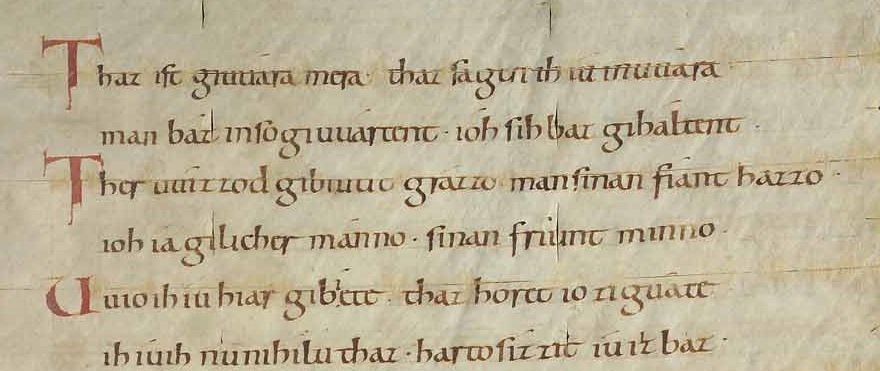
\includegraphics[width=10 cm]{images/otfrid-handschrift-ausschnitt.jpg}
  \caption {Die Anfangszeilen von Otfrids Evangelienbuch}
\label{abb:otfrid-hand}
\end{center}
\end{figure} 

% In schwarz-weiß: images/otfrid-handschrift-ausschnitt-sw.jpg

%http://diglib.hab.de/mss/131-1-extrav/start.htm?image=00007
% Nutzung: CC-BY-SA
% http://diglib.hab.de/copyright.html

Für syntaktische Untersuchungen ist der Text nicht ganz unproblematisch, da die Sprache an vielen Stellen durch Reim und Metrik beeinflusst wird. Ein eindeutiges Ergebnis von  Reimzwang sind \textcite[35--36]{Fleischer2006} zufolge z.B. Kongruenzformen von Partizip\,+\,\object{wësan}, die ausschließlich bei Otfrid zu beobachten sind \parencites()()[s. auch][52]{Fleischer2011}[]{Gillmann2016}. 
Die Wortstellung ist oft rhythmischen Prinzipien untergeordnet: So stehen attributive Adjektive und Determinierer häufiger als in anderen Schriftstücken postnominal \parencites()()[282--283]{Oubouzar1989}[29]{Schrodt2004}. Und auch bei der Setzung von \object{dër} dürfen metrische Gründe (ähnlich wie  \textcite{Eggenberger1961} sie etwa für den Gebrauch des Sub"-jekts"-pronomen postuliert) nicht ausgeschlossen werden. Wie \textcite[37]{Fleischer2006} anmerkt, ist es allerdings schwierig, diese stilistischen Einflüsse methodisch aufzuspüren. In der vorliegenden Untersuchung werden Reim und Metrum daher als mögliche Ursachen für Auffälligkeiten in der Nominalsyntax gewertet, aber nicht explizit als Variablen annotiert. Was die Analyse der funktionalen Spannweite von \object{dër} angeht, ist Otfrids Evangelienbuch sehr gut geeignet, da keine lateinischen Interferenzen die Sprache beeinflussen. 

\subsection{Notkers Boethius} \label{sec:notker}

Notker III. (auch: Notker Labeo) ist Urheber der umfangreichsten Textsammlung, die aus dem späten Ahd. überliefert ist \parencites[157]{Meineke2001}. In seiner Rolle als Lehrer an der Klosterschule St. Gallen übertrug Notker nicht nur theologische, sondern auch wissenschaftliche und philosophische Texte aus der Antike ins Althochdeutsche und zwar mit dem Ziel, daraus Lese- und Interpretationsgrundlagen zu schaffen \parencite[zur Übersicht s.][136]{Sonderegger2003}. Für die nachfolgende Untersuchung wird Buch 1 und 2 von Notkers Boethius-Übersetzung \hervor{De consolatione Philosophiae} als Textgrundlage gewählt. Es handelt sich hierbei um einen Dialog zwischen dem Autor Boethius (5.-6. Jh.) und der personifizierten Philosophie \parencite[vgl.][]{Gruber2006}, der um 1025 von Notker übersetzt wurde \parencite[138]{Sonderegger2003}. 
In Abbildung~\ref{abb:notker-hand}\footnote{St. Gallen, Stiftsbibliothek, Cod. Sang. 825, p. 6 – Boethius, De consolatione philosophiae; \url{https://www.e-codices.ch/de/csg/0825/6/0/Sequence-673}; zuletzt aufgerufen am 12.02.2020.} sieht man, wie sich lateinische Grund- und althochdeutsche Zielsprache zeilenweise abwechseln.   

 \begin{figure}[h]
\begin{center}
  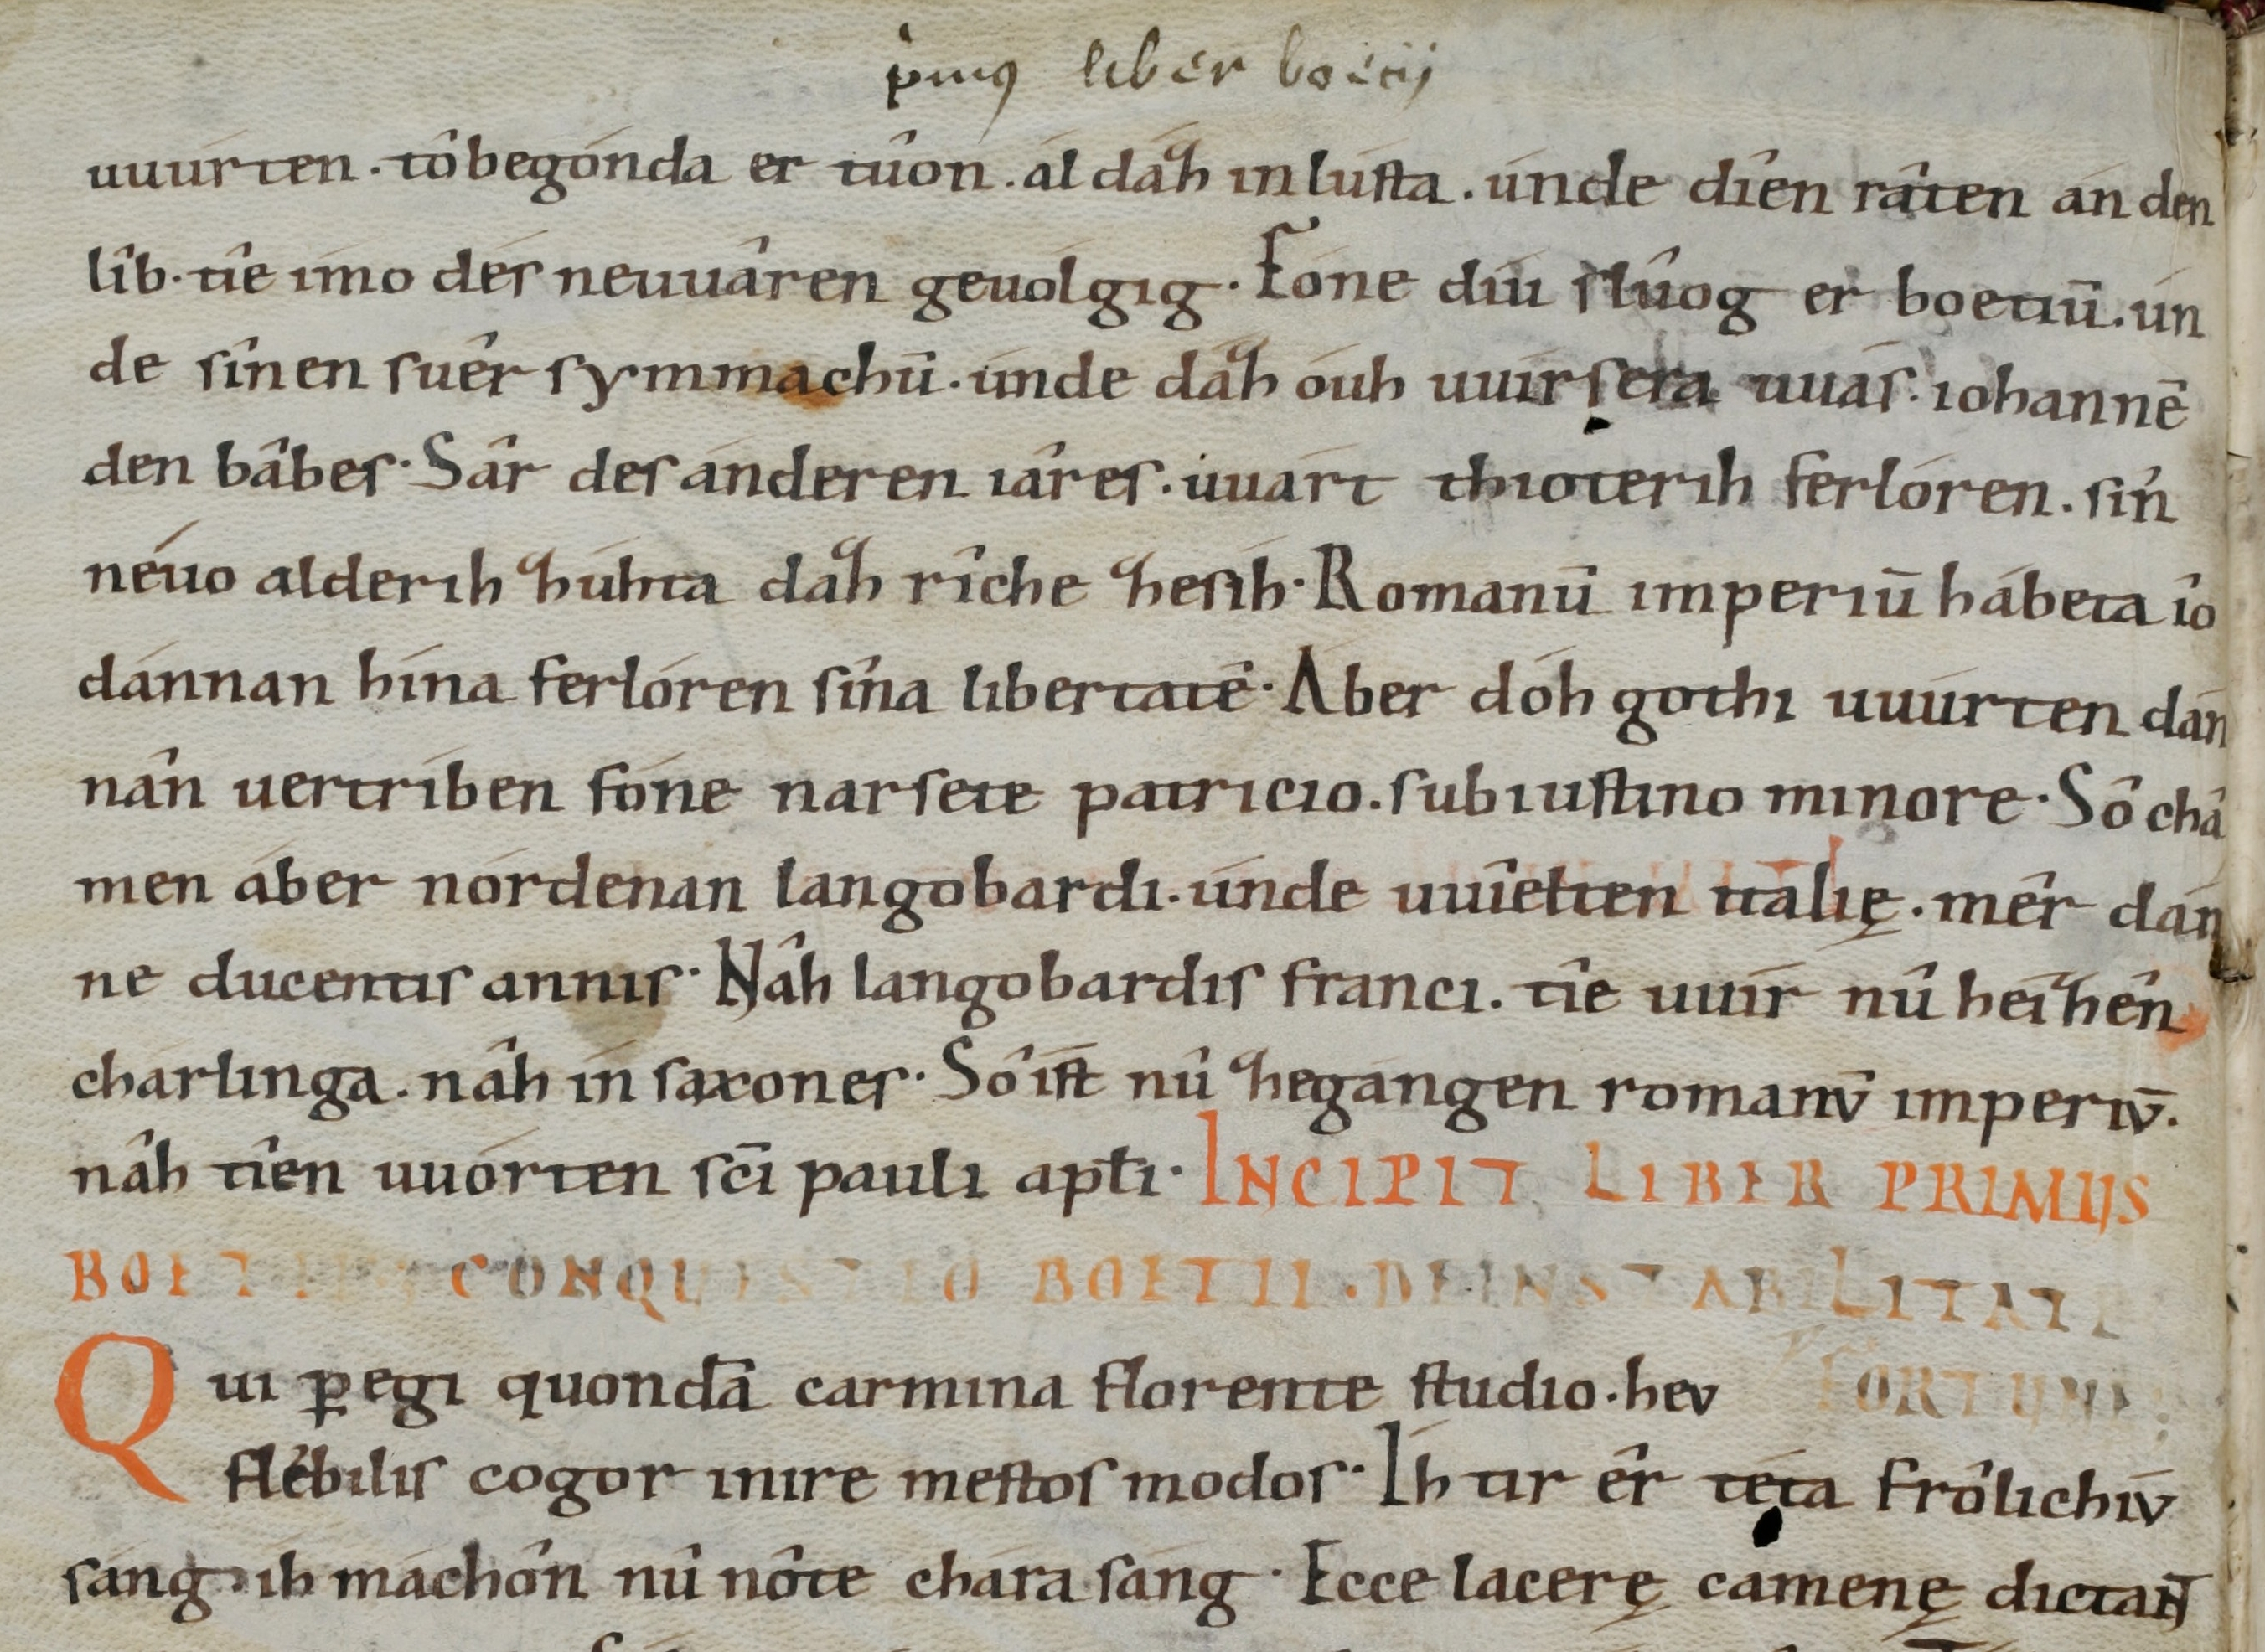
\includegraphics[width=10 cm]{images/notker-handschrift-buch1-ausschnitt.jpg}
\caption {Auszug aus Notkers Boethius, Buch 1}
\label{abb:notker-hand}
\end{center}
\end{figure} 

%In schwarz-weiß: notker-handschrift-buch1-ausschnitt-sw.jpg

Wie variabel Notker in seiner Übersetzung ist, dokumentiert die Studie von \textcite{Eilers2003}; zu Notkers Übersetzungstechnik s. auch \textcite{Glauch2003}. So werden bei der Übersetzung Satzteile oder ganze Sätze (vor allem Nebensätze) eingefügt, umgestellt oder auch getilgt, um ein besseres Textverständnis zu erzielen. Darüber hinaus ergänzt Notker die Vorlage mit eigenständigen ahd. Kommentaren. Um den ahd. Text im Lateinischen zu verankern, sind diese kommentierenden Passagen allerdings manchmal mit lat. Zitaten versetzt \parencite[vgl.][137]{Sonderegger2003}, was einem \blockcquote{Glaser2016}{mittelalterlichen Codeswitching} gleichkommt und die syntaktische Analyse erschwert.  


\section{Datenaufbereitung} \label{sec:datenaufbereitung}

Anders als in den bisherigen Studien zum Definitartikel konnte bei der vorliegenden Untersuchung auf die annotierten Daten des \herkur{Referenzkorpus Altdeutsch} zugegriffen werden. Nachfolgend wird zunächst das Korpus beschrieben (\ref{sec:ddd}) und dann erläutert, welche Schritte notwendig waren, um die Daten in ein weiterverarbeitbares Format zu überführen (\ref{sec:aufbereitung}). Der daran anschließende Abschnitt dokumentiert, auf welche Art und Weise die Annotation vonstatten ging und welche Richtlinien ihr zugrunde lagen (\ref{sec:annotationsschritte}).

\subsection{Das \object{Referenzkorpus Altdeutsch}} \label{sec:ddd}

Die in den vorhergehenden Abschnitten beschriebenen Texte sind über das \object{Referenzkorpus Altdeutsch} \parencite{Donhauser2015} zugänglich. In der vorliegenden Untersuchung wurde mit einer Vorversion von Version 0.1 des Korpus gearbeitet \parencite{Donhauser2014}. Diese Version enthält neben den besagten Schriftstücken alle Textdenkmäler, die aus der althochdeutschen und altsächsischen Sprachperiode überliefert worden sind; die Texte beruhen auf handschriftennahen Editionen und umfassen etwa 300.000 Wortformen.
Die Texte wurden im Rahmen eines DFG-Projekts\footnote{Die Projektleitung für das DFG-geförderten Projekt (2008--2014) unterlag Karin Donhauser (HU Berlin), Jost Gippert (Frankfurt) und Rosemarie Lühr (Jena).} tokenisiert, lemmatisiert und übersetzt. Darüber hinaus sind sie nach Wortarten annotiert\footnote{Tagset DDDTS = Deutsch Diachron Digital Tagset.} und mit flexionsmorphologischen Kategorien gekennzeichnet; neben tokenspezifischen Informationen (z.B. Kasus, Numerus) wurde auch die Flexionsklassenzugehörigigkeit des Lemmas vermerkt (z.B. starke/schwache Flexion). Zusätzlich liefert das Korpus strukturelle Annotationen (Kapitel, Zeile, Vers etc.) zu den einzelnen Texten. 


\subsection{Export aus ELAN und Aufbereitung mit R}\label{sec:aufbereitung}

Um die ausgewählten Texte aus dem Altdeutschkorpus mit eigenen Annotationen anzureichern und die Belege  statistisch auswerten zu können, mussten sie in ein bearbeitbares Format überführt werden. Für die vorliegende Untersuchung wurde das Dateiformat CSV gewählt. CSV-Dateien sind mit den meisten Programmen kompatibel und gewähren eine nachhaltige Datenspeicherung. 

Zum Zeitpunkt der Untersuchung (Anfang 2015) war es nicht möglich, die Texte in ihrer Gesamtheit als CSV-Dateien aus ANNIS3 \parencite{Krause2016}, der Plattform, über die die Texte öffentlich zugänglich sind, zu exportieren.\footnote{Über ANNIS3 kann man zwar Abfragen und Auswertungen durchführen, jedoch keine weiteren Annotationen hinzufügen oder komplexere Auswertungen (etwa statistische Tests) vornehmen, s. \url{https://korpling.german.hu-berlin.de/annis3/}; zuletzt aufgerufen am 12.02.2020.} Das Material wurde mir vom Altdeutsch-Projekt in Form von EAF-Dateien (=\,\object{ELAN Annotation Format}) zur Verfügung gestellt\footnote{Ein besonderer Dank gilt an dieser Stelle Martin Klotz für die Bereitstellung der Texte.}, welche mit ELAN\footnote{\url{https://tla.mpi.nl/tools/tla-tools/elan/}; zuletzt aufgerufen: am 12.02.2020.} in CSV-Dateien konvertiert werden konnten. 
Das Skript \hervor{aufbereitung-rohdaten.R} in \textcite{HZKYL4_2020} dokumentiert, wie Fehler, die durch den Export entstanden sind, korrigiert wurden und welche weiteren Aufbereitungsschritte mithilfe von R\footnote{Version: 3.2.3 (2015-12-10); \url{https://www.R-project.org/}; zuletzt aufgerufen am 12.02.2020.} vorgenommen wurden. 
Um die Annotationen für Kongruenzabfragen und statistische Auswertungen zu nutzen, war es bspw. notwendig, die morphologischen Informationen aus dem Korpus als einzelne Variablen \hervor{auszulagern}. So wurden im Altdeutsch-Projekt die adjektivischen Flexionskategorien in einer Variable (als String) \hervor{pos\_neut\_sg\_acc\_wk} annotiert. Diese fünf Kategorien (Komparation, Genus, Numerus, Kasus und starke/schwache Flexion) mussten gesplittet und in je eine neue Variable überführt werden. Außerdem wurden eine Reihe von Hilfsvariablen angelegt, um Strukturtypen der Nominalphrase aus den Daten auslesen zu können; die entsprechenden Befehle sind ebenfalls in dem o.g. Skript aufgeführt.  

\subsection{Annotationsschritte}\label{sec:annotationsschritte}

Für die Untersuchung wurden folgende Ebenen annotiert: Belebtheit, Relevanz, semantische Rollen, Struktur der Nominalphrase und Definitheitskontexte. Die Belebtheits- und Relevanzannotation erfolgte auf Basis der Übersetzungen, die im Altdeutschkorpus bereitgestellt wurden (=\,Konzeptbasierte Annotation); die anderen Annotationen operierten auf den ahd. Token  (=\,Tokenbasierte Annotation). Nachfolgend werden die Annotationstiefe sowie die einzelnen Vorgehensschritte erläutert, wobei die Belebtheitsannotation den methodischen Hauptteil der Arbeit darstellt und somit den größten Raum einnimmt. Der Leitfaden zur Annotation der einzelnen Kategorien und die dazugehörigen Daten sind in \textcite{HZKYL4_2020} dokumentiert. 

%\subsubsection{(a) Belebtheit} 

Bislang sind in der Sprachwissenschaft kaum Studien zu finden, in denen authentische Daten systematisch nach Belebtheit annotiert wurden und die somit als Vorbild für die komplexe  Belebtheitsannotation dienen könnten. Die Erkenntnisse sprachtypologischer Forschungen (vgl. Kapitel \ref{chapter:belebtheit}) basieren auf Einzelbelegen oder auf konstruierten Beispielen aus Grammatiken \parencite[z.B.][]{Comrie1989,Corbett2000,Aissen2003}. Die wenigen existierenden Korpusuntersuchungen  \parencite{Dahl1996,Yamamoto1999} machen keine Angaben, nach welchen Richtlinien annotiert wurde.

Pionierarbeit zur Belebtheitsannotation wurde im Bereich der historischen Linguistik im Rahmen des DFG-Projekts \hervor{Entwicklung der satzinternen Großschreibung im Deutschen (SiGS)} \parencite[vgl.][]{Szczepaniak2016} geleistet. Auf Basis der im Projekt ausgearbeiteten Richtlinien\footnote{Für die Bereitstellung danke ich Renata Szczepaniak und allen Mitarbeiterinnen und Mitarbeitern im SiGS-Projekt.} wurde eine eigene Anleitung zur Belebtheitsannotation für die vorliegende Untersuchung entwickelt. Darüber hinaus flossen die in Abschnitt \ref{sec:konabst} angesprochenen theoretischen Erkenntnisse zur Semantik von Substantiven im Deutschen \parencite[u.a.][]{Ewald1992,Studler2011} in die Annotationsrichtlinien ein sowie  Vorarbeiten aus der Computerlinguistik mit ein \parencite[vgl.][]{Garretson2004,Zaenen2004,Ovrelid2009}. HIer sind Belebtheitsannotationen bereits seit einigen Jahren Gegenstand des wissenschaftlichen Diskurses. Abbildung~\ref{abb:belebtheitsannotationsschema} gibt einen Überblick über die Kategorien, die bei der Annotation unterschieden wurden.

\begin{sidewaysfigure}
\small
% % 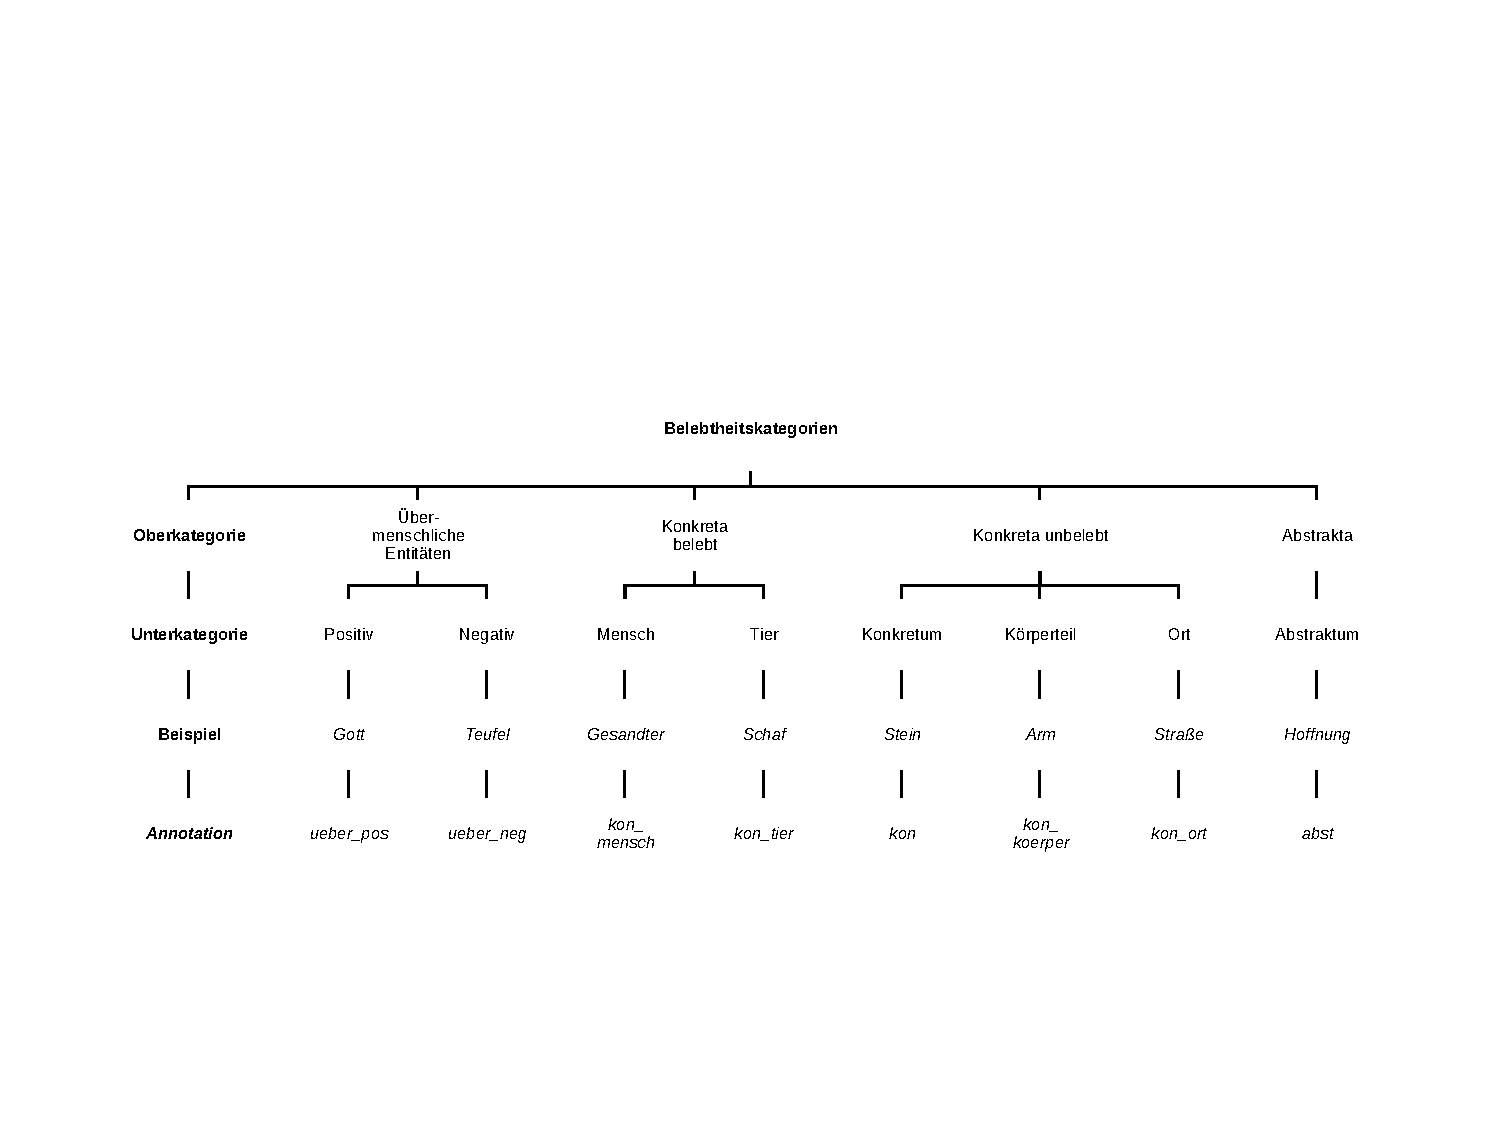
\includegraphics[width=\textwidth]{images/annotationsschema.pdf}
\begin{forest}
forked edges,for tree={fit=tight}
[Belebtheitskategorien,font=\bfseries
    [Oberkategorie,font=\bfseries,for descendants={font=\bfseries} 
                               [Unterkategorie [Beispiel [\itshape Annotation]]]]
    [Übermenschliche Entitäten [Positiv [\textit{Gott} [\textit{ueber\_pos}]]]
                               [Negativ [\textit{Teufel} [\textit{ueber\_neg}]]]
    ]
    [Konkreta belebt [Mensch [\textit{Gesandter} [\textit{kon\_mensch}]]]
                     [Tier [\textit{Schaf} [\textit{kon\_tier}]]]
    ]
    [Konkreta unbelebt [Konkretum [\textit{Stein} [\textit{kon}]]]
                       [Körperteil [\textit{Arm} [\textit{kon\_koerper}]]]
                       [Ort [\textit{Straße} [\textit{kon\_ort}]]]
    ]
    [Abstrakta [Abstraktum [\textit{Hoffnung} [\textit{abst}]]]]
]
\end{forest}
\caption {Belebtheitsannotationsschema\label{abb:belebtheitsannotationsschema}}
\end{sidewaysfigure} 

Vertikal abgebildet sind Ober- und Unterkategorien sowie je ein Beispiel und der zugehörige \object{Tag}. Horizontal finden sich die Belebtheitskategorien und zwar absteigend von links [+belebt] nach rechts [\textminus{}belebt],  wobei teilweise weitere kognitive Faktoren die Unterteilung überlagern: So bildet die Hierarchie auch Aspekte der kulturellen Relevanz ab, da ganz links die sog. \object{übermenschlichen} Referenten stehen. Bezeichnungen für Orte sind prädestiniert dafür, eine niedrige Individualität bzw. Spezifizität aufzuweisen, da sie oft als Adverbial fungieren.\footnote{Bei den Konkreta wurden darüber hinaus Körperteile gesondert annotiert. Diese Gruppe ist allerdings weniger für die Belebtheit relevant, sondern in Bezug auf die Frage, inwiefern der emergierende Artikel bereits in nicht-demonstrativen Definitheitskontexten gebraucht wird (vgl. Abschnitt \ref{sec:pragsem}).} Viele Referenten sind -- wie die Ausführungen in Abschnitt \ref{sec:konabst} gezeigt haben~-- zwischen dem Pol [abstrakt] und [konkret] anzusiedeln. Um dieser Gruppe gerecht zu werden, wurde eine Zwischenkategorie angesetzt. Der Belebtheitsleitfaden enthält eine detaillierte Anleitung mit Beispielen, mit dem Ziel, eine möglichst objektive Zuordnung zu gewährleisten.

Vor der Annotation musste die Frage geklärt werden, ob lexem- oder token"-basiert annotiert wird. Für eine tokenbasierte Annotation spricht, dass so auch Referenzverschiebungen durch Metaphern und Metonymien sowie kontextspezifische Interpretationen einbezogen werden können (\object{die Seiten im Buch} vs. \object{beide Seiten haben recht}). \textcite{Ovrelid2009} zeigt in einem Vergleich von Lexem- und Token\-annotation in schwedischen Wissenschaftstexten, dass solche Referenzverschiebungen mit 1,1\%  allerdings vergleichsweise selten sind.  Bei biblischen Texten, die naturgemäß einen höheren Anteil an Gleichnissen und metaphorischen Bezügen aufweisen, etwa falsche Propheten als \object{Wölfe} oder das Volk als \object{Schafsherde}, sieht die Verteilung jedoch vermutlich anders aus. 

Eine Art Kompromiss zwischen Lexem- und Tokenannotation ergibt sich,\linebreak wenn man die Übersetzungen, die im Altdeutsch-Projekt angefertigt wurden, als Annotationsgrundlage nimmt.  
Über den Internetauftritt des Projekts erfährt man: \hervor{Die Ebene \object{translation} enthält eine zum inhaltlichen Kontext des Lemmas passende Auswahl aus den bei \textcite{Splett1993} gegebenen Übersetzungsvorschlägen zum Lemma.}\footnote{\url{https://www.deutschdiachrondigital.de/manual/annotationsebenen}; zuletzt aufgerufen am 12.02.2020.} Konkret heißt dies, dass dasselbe Lemma je nach Kontext unterschiedlich übersetzt wurde.\footnote{Es muss angemerkt werden, dass -- wie mir Sonja Linde aus dem Projekt mitteilte -- die Übersetzungen nicht Teil der wissenschaftlichen Korpusarbeit waren und an vielen Stellen auch andere Lesarten möglich sind, da kein Leitfaden für die Übersetzungen entwickelt wurde. Eine systematische Kontextanalyse der ahd. Token bleibt somit noch ein Forschungsdesiderat.} So wird das Lemma \object{wahsmo} in einigen Kontexten mit \extrans{Frucht} oder \extrans{Schößling, Sproß} übersetzt und verweist damit auf einen konkreten Referenten. In anderen Fällen lautet die Übersetzung \extrans{Frucht, Kraft, Wachstum}, was einer  abstrakten (metaphorischen) Lesart von \object{wahsmo} Rechnung trägt. Umgekehrt kann ein und dieselbe Übersetzung, d.h. ein bestimmtes semantisches Konzept, für unterschiedliche Lemmata stehen, z.B. \hervor{Gleichnis} für ahd. \object{wortbilidi}, \object {gilīhnissi, gilīhnissī} oder \object{rātissa}. Indem man die Belebtheitsannotation auf Basis der Übersetzungen durchführt, kommt man einer kontextspezifischen Belebtheitsannotation also sehr nahe, vgl. zur Illustration Tabellen~\ref{tab:uem:1} und~\ref{tab:uem:2}. 
Ein wichtiger Vorteil dieser Annotationsform besteht zudem darin, dass große Datenmengen analysiert werden können, da nicht alle Token einzeln annotiert werden müssen und die Annotation auch ohne Althochdeutschkenntnisse erfolgen kann.


\begin{table}
\caption {Übersetzungsmöglichkeit im Altdeutschkorpus (1): Das gleiche Lemma wird unterschiedlich übersetzt.\label{tab:uem:1}}
\begin{tabular}{llll}
\lsptoprule
Token & Lemma & Übersetzung & Belebtheit\\\midrule
uuahsmo & \ldelim\{{3}{1em}[wahsmo] & Frucht & kon\\
uuahsmon & & Frucht, Kraft, Wachstum & abst\\
uuahsmon & & Schößling, Sproß & kon\\
\lspbottomrule
\end{tabular}
\end{table}

\begin{table}
\caption {Übersetzungsmöglichkeit im Altdeutschkorpus (2): Unterschiedliche Lemmata werden gleich übersetzt.\label{tab:uem:2}}
\begin{tabular}{llll}
\lsptoprule
Token & Lemma & Übersetzung & Belebtheit\\\midrule
uuortbilidin & wortbilidi & \rdelim\}{3}{1em}[Gleichnis] & abst\\
gilihnessi & gilīhnissi, gilīhnissī &  & abst\\
ratissa & rātissa &  & abst\\
\lspbottomrule
\end{tabular}
\end{table}

% % % \begin{figure}
% % % \begin{center}
% % %   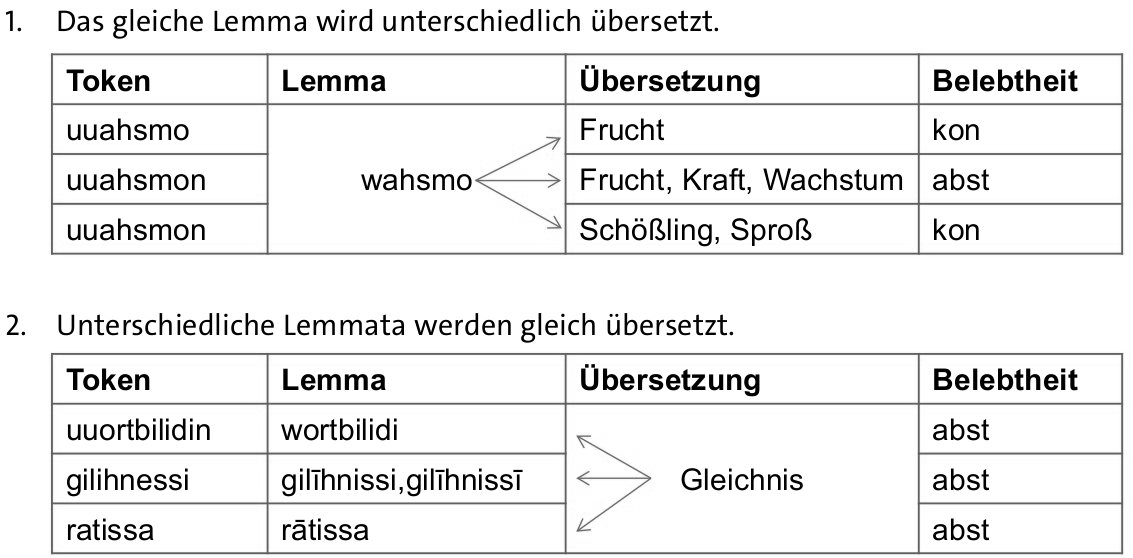
\includegraphics[width=10 cm]{images/konzept-ddd-sw.jpg}
% % % \caption {Übersetzungsmöglichkeiten im Altdeutschkorpus}
% % % \label{abb:konzept-ddd}
% % % \end{center}
% % % \end{figure} 
 

Der Annotationsprozess bestand aus einem zyklischen Wechsel von Annotation, Eva"-lu"-ation, Ergebnisdiskussion und Anpassung des Leitfadens \parencite[entsprechend dem aus der Computerlinguistik bekannten \object{MAMA cycle} (=\,\herkur{Mod"-el-An"-no"-tate-Mo"-del-An"-no"-tate}), beschrieben u.a. in][109]{Pustejovsky2012}.

In einer Pilotstudie wurde eine Liste aller Übersetzungen (den Konzept-Types) erstellt, die entweder als Appellativa oder Eigennamen getaggt waren. Als Datengrundlage wurden der ahd. Isidor, der Tatian und Otfrids Evangelienharmonie genommen.  
Tabelle~\ref{tab:konzept-types} illustriert einen Ausschnitt der generierten Liste, welche 5195 Types umfasste. Die Länge der Liste resultierte nicht nur aus den unterschiedlichen Kontexten, sondern auch aus Variationen in der Zeichensetzung, z.B. Aufzählung mit Komma oder Semikolon, und Tippfehlern.  

\begin{table}
\centering
\begin{tabular}{l}
\lsptoprule
\multicolumn{1}{c}{Übersetzung (Konzept-Type)}    \\ \midrule
Bote                                        \\
Bote, (Ab)gesandter                         \\
Bote, Engel                                 \\
Bote, Gesandter                             \\
Bote, Herold                                \\
Bote, Herold, (Ab)gesandter, Apostel, Engel \\
Bote, Herold, (Ab)gesandter, Engel          \\
Bote, Herold, Engel                         \\
...                                         \\ \lspbottomrule
\end{tabular}
\caption{Auschnitt aus der der Konzept-Type-Liste\label{tab:konzept-types}}
\end{table}

Es folgte eine Probeannotation mit drei Annotatorinnen\footnote{Neben meiner Person waren dies Lisa Bürgerhoff und Jana Giesenschlag, für deren Hilfe ich mich an dieser Stelle herzlich bedanke.} auf Basis einer ersten Version des Belebtheitsleitfadens. Ausgewählt wurden die ersten 508 Übersetzungen (von \object{Aas} bis \object{Bote}) aus der Liste; die Annotation dauerte ca. 60 Minuten. Das \herkur{Inter Annotator Agreement} der drei Annotationen wurde mittels Fleiss' Kappa gemessen \parencite{Fleiss1971}. Das Maß nimmt Werte zwischen 0 und 1 an. 
0 steht für eine niedrige Übereinstimmung, die bei zufälliger Annotation erwartbar wäre, 1 steht für perfekte Übereinstimmung. Zur detaillierteren Interpretation der Werte wurde die Skala von \textcite{Landis1977} herangezogen, s. Abbildung~\ref{abb:kappa-skala}.\footnote{Zu weiteren Interpretationsmöglichkeiten des Kappa-Koeffizienten vgl. die Diskussion in \textcite[576--577]{Artstein2008}.}

\begin{table}
\centering
\label{tab:iaa-pilot}
\begin{tabular}{lc}
\lsptoprule
Annotatorinnen & Fleiss' Kappa  \\ \midrule
A1 und A2               & 0,686  \\
A1 und A3               & 0,721  \\
A2 und A3               & 0,759  \\
A1, A2 und A3           & 0,722  \\ \lspbottomrule
\end{tabular}
\caption{\herkur{Inter Annotator Agreement} der Belebtheitsannotation (Pilotannotation mit drei Annotatorinnen)}
\end{table}

\begin{figure}
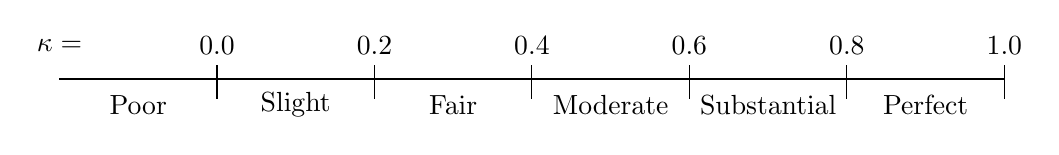
\begin{tikzpicture}[
        /pgf/number format/.cd,
		fixed,
		precision=1, 
		fixed zerofill,
		every node/.style={font=\strut}
    ]
	\node at (-2,0) {$\kappa=$};
	\draw (-2,-\baselineskip) -- (10,-\baselineskip);
	\foreach \i in {0,2,4,6,8,10}
		{
		   \node at (\i,0) {\pgfmathparse{\i/10}\pgfmathprintnumber{\pgfmathresult}};
		   \draw  (\i,-.25) -- ++(0,-\baselineskip);
		};
	\foreach \x/\y in {-1/Poor, 1/Slight, 3/Fair, 5/Moderate, 7/Substantial, 9/Perfect}
		{
		  \node at (\x,-.75) {\y};
		};
	\end{tikzpicture}
\caption {Kappa-Werte und Stärke der Übereinstimmung \parencite[576]{Artstein2008}\label{abb:kappa-skala}}
\end{figure} 

In diesem ersten Durchgang wurde mit einem Kappa-Wert von 0,722 (\herkur{substantial}) bereits eine relativ hohe Übereinstimmung zwischen den drei Annotationen erzielt, vgl. Abbildung~\ref{abb:kappa-skala}. 
Nach einer intensiven Auseinandersetzung mit systematischen Fehlern\footnote{Zur Diskussion stand bspw., ob Körperflüssigkeiten als Körperteile zu definieren sind.} wurde der Leitfaden überarbeitet und erneut ca. 500 Konzept-Types doppelt annotiert. Diesmal geschah die Annotation allerdings unter Ausschluss von Eigennamen, weil diese für die spätere Analyse wenig relevant sind, aber einen relativ großen Teil der Konzept-Type-Liste ausgemacht haben und für eine hohe Übereinstimmung sorgten. Denn Eigennamen verweisen meist auf eindeutig menschliche Referenten (etwa \object{Andreas, Aaron}) oder Städte (z.B. \object{Babylon, Bethlehem}).
Ihr Wegfall hatte dann vermutlich zur Folge, dass beim zweiten Durchgang der Kappa-Wert mit 0,552 deutlich unter dem ersten Wert lag. 
Die Konfusionsmatrix in Abbildung~\ref{abb:confusion} zeigt, dass im zweiten Durchgang vor allem zwischen den Abstrakta, den Konkreta und der Zwischenkategorie \hervor{abstrakt/konkret} Uneinigkeit herrschte. 
Vermutlich ist der Kappa-Wert bei \textcite{Zaenen2004} höher (sie erzielten bei ihrer Belebtheitsannotation einen Wert über 0,9), weil sie nur zwischen prototypisch konkret und nicht-konkret differenzieren. Man sieht auch, dass Annotatorin 1 (horizontal) entscheidungsfreudiger war als Annotatorin 2 (vertikal), da letztere häufiger ein \hervor{unklar} vergab. Interessant ist hier die Kategorie \hervor{kon\_ort}, in welche Annotatorin 1 Konzept-Types wie \object{Erde, Haus}, \object{Erde, Gebiet} oder \object{Einöde, Wüste} eingeordnet hat, während von Annotatorin 2 hier \hervor{abst\_kon} oder \hervor{abst} annotiert wurde. In Zukunft könnte man durch eine intensive \hervor{Fehler}-Analyse solcher Annotationsdurchgänge weitere Erkenntnisse für Belebtheitsannotationen ableiten.  
 
\begin{figure}
\begin{center}
  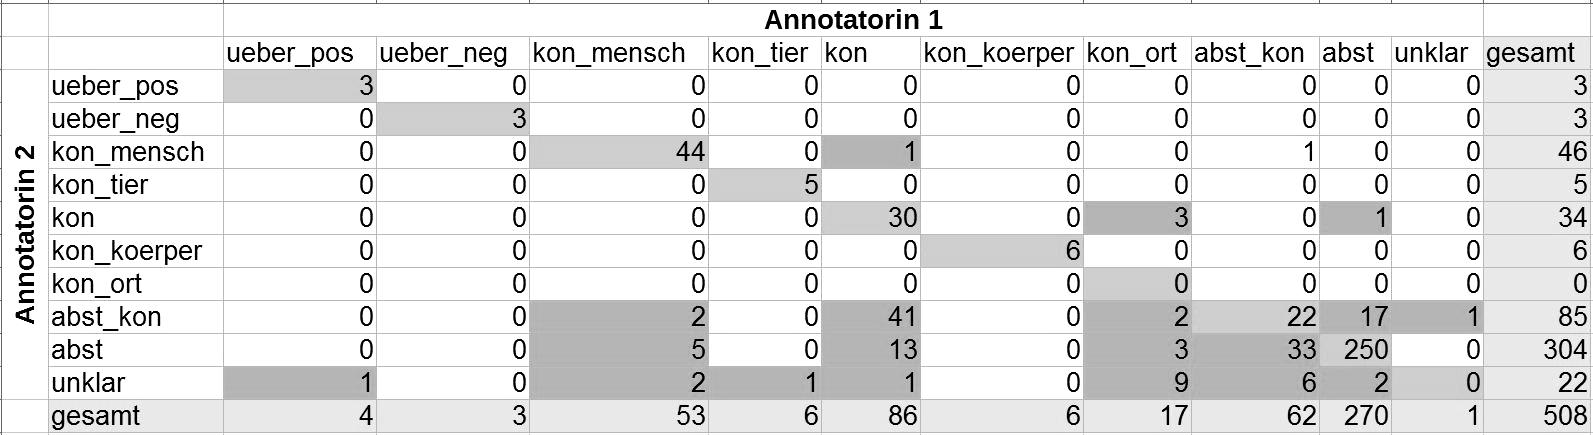
\includegraphics[width=12 cm]{images/confusionsmatrix-neu-sw.jpg}
\caption {Konfusionsmatrix für die zweite Annotationsrunde}
\label{abb:confusion}
\end{center}
\end{figure} 

Für den dritten und letzten Annotationsdurchgang wurde der Leitfaden erneut leicht angepasst.\footnote{Die finale Version des Leitfadens liegt in \textcite{HZKYL4_2020} ab.} Die Konzeptliste wurde nach dem Modell des vorhergehenden Durchgangs (also ohne Eigennamen), aber diesmal auf Basis aller zu untersuchenden Texte (s. Abschnitt \ref{sec:textauswahl}), erstellt (=\,15.039 Types) und doppelt annotiert.\footnote{Da auch Buchstaben oder Satzzeichen unter der Liste zu finden waren, wurden diese vor der Annotation mit \hervor{keine Angabe} gekennzeichnet.} Der neue Kappa-Wert lag bei 0,701. Übersetzungen, die aus Verständnisgründen als \hervor{unklar} klassifiziert wurden und deswegen nicht nach Belebtheitheit annotiert werden konnten, wurden von mir mit Erklärungen versehen und anschließend erneut zur Annotation freigegeben. Der Kappa-Wert veränderte sich hierdurch nur unwesentlich (0,688); insgesamt ist die Übereinstimmung mit Blick auf Abbildung~\ref{abb:kappa-skala} also als  \herkur{substantial} zu werten. Für die Auswertung wurden am Ende nur die Fälle einbezogen, bei denen beide Annotatorinnen übereinstimmten.

%\subsubsection{(b) Relevanz} 

Bei der Belebtheitsannotation wurde der Faktor Relevanz mit der Kategorie "übermenschliche Entitäten" (s. Abbildung~\ref{abb:belebtheitsannotationsschema}) in Teilen schon abgedeckt. Um zu überprüfen, inwiefern das Geschlecht einen Einfluss auf den Artikelgebrauch hat, wurden zusätzlich alle menschlichen Konkreta in [männlich] und [weiblich] unterteilt.\footnote{Bei dieser Aufgabe habe ich Untertützung von Lisa Bürgerhoff erhalten.} 
Trotz der recht eindeutigen Dichotomie gibt es durchaus Fälle, die in die Klasse \hervor{unklar} fielen, z.B. \object{Mitbürger} oder \object{Altersgenossen}, welche bei der Analyse dann ausgespart wurden.  Die Annotation erfolgte erneut konzeptbasiert, d.h. die Grundlage bildete eine automatisch generierte Liste von Übersetzungen, die am Ende wieder mitsamt der \hervor{Geschlechtsannotation} den jeweiligen ahd. Token zugeordnet wurden. 

%\subsubsection{(d) Struktur der Nominalphrase}

Um die Struktur der Nominalphrase zu annotieren, wurde eine zufällige Stichprobe\footnote{Zum Vorgehen vgl. das R-Skript \hervor{aufbereitung-rohdaten.R} auf Trollling (Todo: URL einpflegen.} (bestehend aus je 100 Appellativa) aus dem Isidor, dem Tatian und Otfrid genommen. Annotiert wurden Informationen zum Phrasentyp und zur Art und Anzahl von Determinierern sowie Attributen. 
Bei den Übersetzungstexten wurden zusätzlich das lateinische Token und ggf. Abweichungen in der Struktur (Vorhandensein und Stellung von Determinierern und Attributen) dokumentiert. Beim Tatian wurde zudem vermerkt, auf welche Bibelstelle der ahd. Text Bezug nimmt sowie eine Übersetzung davon angegeben. Außerdem gibt es bei der Annotation Raum für Anmerkungen und Übersetzungsprobleme.

%\subsubsection{(e) Definitheit} 
Jede der 100 NPs, die auch strukturell annotiert wurden (vgl. Abschnitt (d), wurde einem Definitheitskontext zugewiesen. Es wurden also nicht nur die in der Stichprobe enthaltenen \object{dër}-Belege nach ihrem Definitheitskontext (pragmatische oder semantische Definitheit) analysiert, sondern auch alle Phrasen ohne \object{dër}, um diese anschließend vergleichen zu können. Die Ausprägungen der Variable \hervor{Definitheit} sind in Tabelle~\ref{tab:definitheit} aufgelistet. Die Kategorien basieren auf \textcite{Lobner1985}, \textcite{Himmelmann1996, Himmelmann1997},  \textcite{Diessel1999}, \textcite{Donhauser2012} und \textcite{Szczepaniak2011a}, vgl. die Gebrauchskontexte in Kapitel \ref{chap:demdef}. Fälle, die nicht eindeutig in eine der Kategorien passten, wurden als \hervor{ambig} gekennzeichnet und später als mögliche Brückenkontexte separat analysiert. 

%\subsubsection{(c) Semantische Rollen} 
Was Art und Anzahl von semantischen Rollen angeht, die als Kandidaten für eine Annotation in Frage kommen, gilt es eine Auswahl aus der Vielzahl von Theorien (vgl. Abschnitt \ref{sec:partizipanten}) zu treffen: Gerade bei historischen Texten stößt man mit jeder neuen Unterkategorie schnell an die Grenzen dessen, was operationalisierbar und damit annotierbar ist. In der vorliegenden Arbeit wurden daher im Rahmen der NP-Stichprobenannotation, die im Abschnitt zuvor beschrieben wurde, Referenten ganz basal in \hervor{Proto-Agens}, d.h. Subjekte, die willentlich handeln,  eine Bewegung ausführen oder Träger eines Gefühlszustandes sind,  und \hervor{Nicht-Proto-Agens} unterteilt.


\begin{table}
\centering
\begin{tabular}{ll}
\lsptoprule
Annotation & Kurzbeschreibung  \\ \midrule
situativ            & Situativer Bezug               \\
anaphorisch         & Anaphorischer Bezug            \\
diskurs             & Diskursdeiktischer Bezug      \\
anamnestisch        & Anamnestischer Bezug           \\
abstrakt            & Abstrakt-situativer Bezug      \\
assoziativ          & Assoziativ-anaphorischer Bezug \\
monoref             & Referent ist monoreferent      \\
generisch           & Generische Lesart              \\
nicht-spezifisch        & Unspezifischer Referent           \\
spezifisch-indefinit          & Spezifischer Referent           \\
indefinit           & Indefinita     \\
possessiv           & Possessiver Bezug    \\
ambig\_kat1\_kat2  & Ambige/Uneindeutige Fälle      \\ \lspbottomrule
\end{tabular}
\caption{Annotationsmöglichkeiten für die Variable \hervor{Definitheit}\label{tab:definitheit}}
\end{table}

\section{Analysemethoden} \label{sec:analysemethoden}

Die Untersuchung fußt auf zwei unterschiedlichen Analysemethoden. Zum einen wurden die in \ref{sec:textauswahl} beschriebenen Texte in ihrer Gesamtheit untersucht, und zwar mithilfe der im Referenzkorpus Altdeutsch vorhandenen Annotationen. Die Daten wurden hierbei nach Einheiten durchsucht, die stellvertretend für das spezifische sprachliche Phänomen stehen, sog. Proxys \parencite[vgl.][114]{Lemnitzer2015}, s. zur Illustration Tabelle~\ref{tab:proxys}. Die Auswahl spezifischer Lexeme, etwa Unika wie \object{sunna} \extrans{Sonne}, orientiert sich an den manuell durchgeführten Vorarbeiten zum Artikelgebrauch. Besonders hervorzuheben sind die Unterschungen von \textcite{Graf1905}, \textcite{Bell1907}, \textcite{Hodler1954} und \textcite{Oubouzar1989}: Hier wurde das ahd. Datenmaterial von Hand nach Belegen durchforstet und ausgezählt. Sie dienen damit als wichtige Referenzquelle für die vorliegende computergestützte Auswertung. 

Zum anderen wurden die Korpusdaten mit eigenen Annotationen angereichert; die Kategorien wurden im vorhergehenden Abschnitt beschrieben. Die Belebtheitsannotation ist so konzipiert, dass sie für eine ganzheitliche Analyse geeignet ist, d.h. alle Appellativa können nach Belebtheit ausgewertet werden. Die Mehrebenen-Annotation zur NP, den Definitheitskontexten und den semantischen Rollen beschränkt sich gemäß ihrer Komplexität und des damit verbundenen Zeitaufwands auf zufällige Stichproben. Bei der Ergebnispräsentation wird jeweils vermerkt, ob die Daten auf Auswertungen des gesamten Korpus oder Stichprobenanalysen basieren. 

\begin{table}
\centering
\begin{tabular}{ll}
\lsptoprule
Kategorie     & Proxy            \\ \midrule
Semantische Definitheit & Superlative, Unika            \\
Definite NP             & Definite Artikelformen\,+\,Nomina Appellativa        \\
Niedrige Individualität & Massennomen, Belege im Plural \\ \lspbottomrule
\end{tabular}
\caption{Operationalisierung unterschiedlicher Kategorien durch Proxys\label{tab:proxys}}
\end{table}
 
\subsection{Qualitative und quantitative Analysen}\label{sec:qual-quant}

Im Normalfall setzen quantitative Auswertungen immer qualitative Entscheidungen voraus.\footnote{Ausnahmen sind Bottom-up-Analysen, die nahezu ohne Einspeisung von theoriegeleitetem Wissen arbeiten, z.B. mithilfe von N-Gramm-Auswertungen wie etwa bei \textcite{Scharloth2012}.} So muss jegliche Information, die ein Korpus zusätzlich zum reinen Primärtext enthält (Tokenisierung, PoS-Tags, morphologische Auszeichnungen, Belebtheitskategorien, Übersetzungen, Meta-Daten etc.) zuvor eindeutig definiert und ggf. für die Annotation operationalisiert werden. Erst dann können die Belege gemäß der Kategorien, in die sie eingeordnet wurden, ausgezählt und statistisch miteinander verglichen werden.   

In der vorliegenden Arbeit basieren die quantitativen Auswertungen auf unterschiedlichen Typen der qualitativen Vorarbeit:
Eine wichtige Grundlage für die Untersuchung bilden die PoS-Annotationen und die morphologischen Informationen, die das Altdeutschkorpus bereitstellt.\footnote{Zur Übersicht der Kategorien s. \url{https://www.deutschdiachrondigital.de/manual/annotationsebenen}; zuletzt aufgerufen am 12.02.2020.} Durch sie können bspw. alle Nomen Appellativa (NAs), denen ein kongruentes \object{dër} (DDA) vorhergeht, ausgezählt werden.

Zudem lassen sich mithilfe der Annotationen sprachliche Muster aufdecken, etwa Kombinationsmöglichkeiten von stark oder schwach flektierten Adjektiven mit \object{dër}. Die einheitliche Lemmatisierung der Texte kann für Stichprobenanalysen genutzt werden, etwa um Gebrauchsunterschiede  von ausgewählten Nomen herauszuarbeiten. So wird der Einfluss von Individualität auf die Artikelsetzung z.B. an Massennomen im Vergleich zu zählbaren Nomen sichtbar.

Die konzeptbasierte Belebtheitsannotation gewährleistet ebenfalls eine globale Analyse der Texte, da jedem Appellativum ein Belebtheitsgrad zugeordnet wird. Auf diese Weise kann der Einfluss der Variable Belebtheit auf die Artikelsetzung überprüft werden. 

Ergänzend zur Analyse der NP-Struktur durch Proxys werden Auswertungen vorgenommen, die auf einer eigenen qualitativen Analyse der NP basieren (s. Abschnitt \ref{sec:annotationsschritte}). Das ahd. Wörterbuch von \textcite{Schutzeichel2012} sowie bisherige Analysen zum ahd. \object{dër} \parencite[v.a.][]{Oubouzar1989} dienen hierbei als Verständnishilfe.  

Um den Einfluss der einzelnen Kategorien auf die Verwendung von \object{dër} zu testen, wurden statistische Signifikanztests ($\chi^2$-Test sowie Exakter Test nach Fisher) und Residuenanalysen (mithilfe von Mosaikplots) durchgeführt \parencite{Gries2012}. Das Signifikanzniveau wurde auf $0,05$ angesetzt.

\subsection{Umgang mit Differenzbelegen}\label{sec:differenz}

Differenzbelege können nicht automatisch, sondern nur manuell klassifiziert\linebreak werden, da zum Zeitpunkt der Untersuchung keine digitale Alignierung von lat. und ahd. Texten vorliegt. Bei der Stichprobenanalyse zur Struktur der NP wurde daher jeder Beleg mit der lateinischen Vorlage von Hand abgeglichen. Alle für die Fragestellung relevanten morphosyntaktischen Abweichungen wurden dokumentiert. Die wichtigsten betreffen a) die Setzung von ahd. \object{dër} und die Frage, ob dies durch ein lateinisches Demonstrativum (v.a. \object{ille}) motiviert sein könnte und b) die Frage nach der Nominalsyntax: Gibt es Stellungsunterschiede bei Determinierern oder Attributen? Für den ahd. Tatian wurde die Edition von Sievers (1966) genutzt, die online über Titus\footnote{\url{http://titus.uni-frankfurt.de/texte/etcs/germ/ahd/tatian/tatia.htm}; zuletzt aufgerufen am 12.02.2020.} eingesehen werden kann. Beim ahd. Isidor konnte auf die lateinische Version im Altdeutschkorpus (Eggers 1964) Bezug genommen werden.  


\section{Zusammenfassung}

In diesem Kapitel wurde gezeigt, wie die Struktur [\object{dër}\,+\,N] im Althochdeutschen über korpuslinguistische Methoden analysiert werden kann. Folgende Texte, deren Herkunft und sprachliche Besonderheiten dargelegt wurden, liegen der Untersuchung zugrunde: Isidor (um 790), Monseer Matthäus (um 810), Tatian (um 840), Otfrids Evangelienbuch (um 870) und Notkers Boethius (1025). Sie wurden im Rahmen des \object{Referenzkorpus Altdeutsch}-Projekt mit grammatischen Informationen (u.a. Wortarten und Flexionskategorien) ausgezeichnet, was eine systematische Suche nach der Zielstruktur [\object{dër}\,+\,N] sowie nach weiteren, für die Fragestellung relevanten Belegstellen, darunter bestimmte Unika, Superlative und Kombinationen von \object{dër}\,+\,Adjektiv ermöglicht. Das methodische Herzstück der Arbeit ist die Belebtheitsannotation, welche in diesem Kapitel schrittweise erläutert wurde. Um eine möglichst objektive Zuweisung der einzelnen Belebtheitsgrade bei den Substantiven zu erreichen, wurde ein Annotationsleitfaden erstellt und die einzelnen Annotationsdurchgänge über \herkur{Inter Annotator Agreements} evaluiert. Auch für die anderen Analysekategorien (Definitheit, Stuktur der NP, semantische Rollen) liegen Richtlinien vor, die im Anhang \parencite{HZKYL4_2020} der Arbeit einzusehen sind. Weil es sich bei einigen Texten um Übersetzungen aus dem Lateinischen handelt, werden auch Differenzbelege, d.h. \object{dër}-Setzungen  und Wortstellungsabfolgen, die von der Vorlage abweichen, gekennzeichnet und separat analysiert. 
  
